\setlength{\columnsep}{3pt}
\begin{flushleft}
	
	\begin{itemize}
		\item CPU stands for \textbf{C}entral \textbf{P}rocessing \textbf{U}nit.
		\item CPU is the brain of the computer. 
		\item CPU is also called as the \textbf{processor}. 
		\item It performs:
		\begin{itemize}
			\item Arithmetic operations such as addition, subtraction etc.
			\item Logical operations i.e. whether something is true or false, etc.
			\item Synchronizes computer operations.
		\end{itemize}
		\item Intel and AMD are leading in processor manufacturing.
	
	\bigskip
	\begin{figure}[h!]
		\centering
		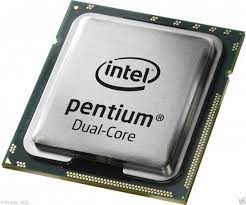
\includegraphics[scale=.5]{content/chapter12/images/cpu.jpeg}
		\caption{Intel dual-core processor}
		\label{fig:process3}
	\end{figure}

\end{flushleft}

\newpage


